% Provenance (never printed): old terminale S material on the transformation of
% rocks in mountain belts and subduction zones (pressure, temperature, index
% minerals and the Al2SiO5 polymorphs, foliation, contact and regional
% metamorphism). Owner (Sync 0): metamorphism, lithostatic pressure, polymorph,
% index mineral/isograd/metamorphic grade, foliation/schistosity, contact and
% regional metamorphism/aureole. Blueschist and eclogite are g11.06's, the
% geotherm g11.03's, minerals and silicates g11.07's, the rock families, marble
% and slate Book 1's (g6), pressure physics': recalled, never redefined. The
% P-T diagram: figdata/grade-12/al2sio5.py (Holdaway and Mukhopadhyay 1993,
% Table 11; geotherms from Earle 7.3).
\chapter{变质岩}\label{ch:g12:metamorphic-rocks}

一层泥沉积于海底，经固结形成页岩。将其埋藏数
千米并加以挤压，便成为板岩，一种能劈成
薄而平的屋顶石板的岩石。再埋得更深、温度更高，其细小的
鳞片长成闪亮的云母，其间红色的石榴石膨大：便是片岩。
埋得更深、温度更高，其矿物按浅色与深色
排列成条带：便是片麻岩。过程中并无熔化。同一种泥，
化学元素不变，只是重新组合其矿物，以适应所在之处。
反过来看，变质岩中的矿物记录了所在之地的深度
与温度，本章将学习如何读取这些记录。
% ledger: earle:foliation, earle:settings

\begin{recall}
岩石分为三大类——火成岩、沉积岩、变质岩——，
岩石循环使三者相互转化；大理岩由石灰岩形成，
板岩由页岩形成，二者均不经熔化（第 1 册，六年级）。矿物是
具有确定化学组成与有序原子排列的天然固体，
地壳中的矿物大多为\omterm{def:g11:minerals:silicate}{硅酸盐}
（见\cref{ch:g11:minerals}）。\omterm{def:g11:lithosphere-asthenosphere:geotherm}{地温线}是某地地下温度随深度变化的曲线，
近地表处温度每千米升高 25 至
\qty{30}{\celsius}（见\cref{ch:g11:lithosphere-asthenosphere}）。
在\omterm{def:g11:subduction-zones:subduction}{俯冲带}中，\omterm{def:g11:ocean-ridges:oceanic-lithosphere}{洋壳}若在低温下被带入地下，
便依次转变为\omterm{def:g11:subduction-zones:eclogite}{蓝片岩}和\omterm{def:g11:subduction-zones:eclogite}{榴辉岩}（见\cref{ch:g11:subduction-zones}）。
压强是力除以其作用面积，
以帕斯卡为单位，\qty{1}{Pa} = \qty{1}{N/m^2}。
\end{recall}
% ledger: usgs:metamorphic (Book 1 row), webmineral:formulas, earle:settings, earle:controls

\section{固态下的转变}

\begin{definition}[变质作用]\label{def:g12:metamorphic-rocks:metamorphism}
\emph{变质作用}\index{变质作用}是指岩石的
矿物与\omterm{def:g11:igneous-rocks:texture}{结构}在固态下发生转变，当其被置于
不同于其形成时的温度与压强之下。
转变后的岩石称为变质岩。
\end{definition}
% ledger: tulane:metamorphism, earle:controls

\omterm{def:g12:metamorphic-rocks:metamorphism}{变质作用}所始于的岩石称为\omterm{def:g10:soil-formation:weathering-profile}{母岩}，
与土壤之下岩石所用的名称相同（见\cref{ch:g10:soil-formation}）。\omterm{def:g12:metamorphic-rocks:metamorphism}{变质作用}始于约 \qty{200}{\celsius}；低于此温度时，埋藏沉积物的缓慢
变化属于其硬结成岩的过程。\omterm{def:g12:metamorphic-rocks:metamorphism}{变质作用}止于
岩石开始熔化之处，此后所发生的属于火成作用。两者之间，
每种矿物仅在一定的温度与压强范围内稳定。
例如，多数\omterm{def:g10:soil-formation:clay}{黏土矿物}仅能稳定至约 150 或 \qty{200}{\celsius}，超过此温度便转变为云母。
当条件改变时，不稳定矿物的原子
逐颗重新排列，
形成在新条件下稳定的矿物。
% ledger: tulane:metamorphism, earle:controls

有四个因素决定变质的结果。\textbf{\omterm{def:g10:soil-formation:weathering-profile}{母岩}}提供
化学元素：仅由方解石构成的石灰岩，只能变成
由方解石构成的大理岩。\textbf{温度}与\textbf{压强}决定哪些
矿物稳定。颗粒之间少量存在的\textbf{水}
携带溶解的离子，自一颗粒传至另一颗粒，并加快
反应。\omterm{def:g12:metamorphic-rocks:metamorphism}{变质作用}进行得很慢，新矿物每百万年约生长一毫米。
埋藏岩石的构造事件同样缓慢，
因此反应通常有足够的时间进行。
% ledger: earle:controls

\subsection{上覆岩石的重量}

埋藏于深度 $z$ 处的岩石承受其上方全部岩石的重量。

\begin{definition}[静岩压力]\label{def:g12:metamorphic-rocks:lithostatic}
\emph{静岩压力}\index{静岩压力}是指深度为 $z$ 处的
岩石所受的压力，即其上方岩柱的重量对该岩石
施加的压力，且各方向上大小相同。
\end{definition}
% ledger: earle:controls (confining pressure, equal in all directions), tulane:metamorphism

\begin{proposition}[静岩压力]\label{prop:g12:metamorphic-rocks:lithostatic}
在密度均匀为 $\rho$ 的岩柱之下，\omterm{def:g12:metamorphic-rocks:lithostatic}{静岩压力}
在深度 $z$ 处为
\[
  P = \rho g z ,
\]
式中 $g$ 为重力加速度；大气压强
约为 \qty{0.1}{MPa}，略去不计。
\end{proposition}

\begin{proof}
取一竖直岩柱，其水平截面积为 $A$，自
地表向下至深度 $z$。其体积为 $Az$，质量为 $\rho A z$，
其重量为 $\rho A z g$。此重量作用于岩柱底部的
面积 $A$ 上，故该处压强为 $P = \rho A z g / A = \rho g z$。
\end{proof}

取\omterm{def:g12:continental-crust:continental-crust}{大陆地壳}的平均密度 $\rho = \qty{2830}{kg/m^3}$，
重力加速度 $g = \qty{9.81}{m/s^2}$，则压强每米增加 $\rho g = 2830 \times 9.81
\approx \qty{27800}{Pa}$，即每千米约
\qty{27.8}{MPa}。在厚度为 \qty{35}{km} 的地壳底部，压强达到
\[
  P = 2830 \times 9.81 \times \num{35000} \approx \qty{9.7e8}{Pa} \approx
  \qty{0.97}{GPa},
\]
约 \qty{1}{GPa}，近万倍于
海平面处的大气压强。压强常可反过来理解为深度：
\qty{1}{GPa} 对应的深度为 $\num{e9}/(2830 \times 9.81) \approx \qty{36}{km}$
地表以下。
% values: P_35km_gpa 0.97168, dPdz_mpa_per_km 27.762, z_1gpa_km 36.02 (al2sio5.py)
% ledger: cm95:crust; Book 1: ussa76:sea-level (101 325 Pa, g0 = 9.80665 m/s2)

岩石的重量从各个方向均匀地施压。在造山带中，
板块在某一方向上施加额外的推力，岩石所受的侧向挤压
比来自上方的更强。这种\emph{定向}压力不改变哪些矿物稳定，
但会改变矿物的排列方式，正如
\cref{sec:g12:metamorphic-rocks:foliation}所示。
% ledger: earle:controls (directed pressure), earle:foliation

\section{指示矿物与变质级}

\subsection{同一化学式的三种矿物}

\begin{definition}[同质多象变体]\label{def:g12:metamorphic-rocks:polymorph}
若两种矿物具有相同的化学组成而晶体\omterm{def:g11:igneous-rocks:texture}{结构}不同，则称它们为
\emph{同质多象变体}\index{同质多象变体}：原子相同，
只是排列方式不同。
\end{definition}
% ledger: earle:controls

三种矿物都具有化学式 \ce{Al2SiO5}：蓝晶石、红柱石
和夕线石。每种矿物各自在一定的温度与压强范围内稳定，
其范围由实验室测定：将晶体置于选定的温度与
压强下，观察哪一种\omterm{def:g12:metamorphic-rocks:polymorph}{同质多象变体}以牺牲另一种为代价而生长。蓝晶石在三者中密度最大，
为 \qty{3.61}{g/cm^3}，夕线石为 \qty{3.24}{g/cm^3}，
红柱石为 \qty{3.15}{g/cm^3}：其原子排列更紧密，它
正是高压所偏好的那一种。
% ledger: earle:controls, hm93:triple, hm93:table11; Book 3: webmineral:polymorphs (densities)

\begin{omfigure}
\begin{tikzpicture}
\begin{axis}[omrecord, name=pt, scale only axis, width=0.62\linewidth, height=6.4cm,
  xmin=200, xmax=900, ymin=0, ymax=1.2, y dir=reverse,
  xlabel={温度 (\unit{\celsius})}, ylabel={压强 (\unit{GPa})},
  xtick={200,300,...,900}, ytick={0,0.2,...,1.2},
  yticklabel style={/pgf/number format/fixed, /pgf/number format/precision=1},
  axis y line*=left]
% computed in figdata/grade-12/al2sio5.py from Holdaway and Mukhopadhyay (1993), Table 11
\addplot[omDef, line width=0.9pt, densely dashed] table[x=T10, y=P_GPa] {figdata/out/grade-12-al2sio5-geotherms.dat};
\addplot[omMeth, line width=0.9pt, densely dashed] table[x=T30, y=P_GPa] {figdata/out/grade-12-al2sio5-geotherms.dat};
\addplot[omThm, line width=0.9pt, densely dashed] table[x=T50, y=P_GPa] {figdata/out/grade-12-al2sio5-geotherms.dat};
\addplot[black, line width=1.2pt] table[x=T, y=P_GPa] {figdata/out/grade-12-al2sio5-andky.dat};
\addplot[black, line width=1.2pt] table[x=T, y=P_GPa] {figdata/out/grade-12-al2sio5-kysil.dat};
\addplot[black, line width=1.2pt] table[x=T, y=P_GPa] {figdata/out/grade-12-al2sio5-andsil.dat};
\addplot[black, line width=1.2pt, dotted] table[x=T, y=P_GPa] {figdata/out/grade-12-al2sio5-andsilx.dat};
\addplot[only marks, mark=*, mark size=2pt, black] coordinates {(504.2,0.3758)};
\addplot[only marks, mark=o, mark size=2pt, line width=0.8pt, black] coordinates {(573.6,0.5216) (340.1,0.1833) (553.0,0.3015)};
\coordinate (ky) at (axis cs:370,0.55);
\coordinate (and) at (axis cs:470,0.12);
\coordinate (sil) at (axis cs:765,0.57);
\coordinate (tp) at (axis cs:504.2,0.3758);
\coordinate (g10) at (axis cs:415,1.0);
\coordinate (g30) at (axis cs:206,0.36);
\coordinate (g50) at (axis cs:895,0.355);
\end{axis}
\begin{axis}[scale only axis, width=0.62\linewidth, height=6.4cm, at={(pt.south west)}, anchor=south west,
  xmin=200, xmax=900, ymin=0, ymax=43.224, y dir=reverse, axis x line=none, axis y line*=right,
  axis line style={-}, ylabel={深度 (\unit{km})}, ytick={0,5,...,40},
  every axis label/.append style={font=\small}, tick label style={font=\small}]
\end{axis}
\node[font=\small\bfseries] at (ky) {蓝晶石};
\node[font=\small\bfseries] at (and) {红柱石};
\node[font=\small\bfseries] at (sil) {夕线石};
\node[font=\scriptsize, text=omDef, anchor=west, inner sep=1pt] at (g10) {\qty{10}{\celsius/km}，俯冲带};
\node[font=\scriptsize, text=omMeth!70!black, anchor=north west, inner sep=1pt, align=left] at (g30) {\qty{30}{\celsius/km}，\\典型};
\node[font=\scriptsize, text=omThm, anchor=south east, inner sep=1pt] at (g50) {\qty{50}{\celsius/km}，火山区};
\end{tikzpicture}

{\small 三种\omterm{def:g12:metamorphic-rocks:polymorph}{同质多象变体}（\ce{Al2SiO5}）的稳定区，压强如深度一样向下增加
（右侧标尺，地壳密度为
\qty{2830}{kg/m^3}）。黑线为实验室测定的边界；
三线相交于三相点（黑点），\qty{504}{\celsius} 与
\qty{0.375}{GPa}。虚线为三条\omterm{def:g11:lithosphere-asthenosphere:geotherm}{地温线}，自地表 \qty{10}{\celsius} 起算；
圆圈标出它们穿过边界的位置。}
\end{omfigure}
% values: triple_T 504.21, triple_P_gpa 0.37584, triple_z_km 13.538; crossings 30: 573.6 degC 18.79 km; 50: 340.1 degC 6.60 km, 553.0 degC 10.86 km (al2sio5.py)
% ledger: hm93:table11, hm93:triple, cm95:crust, earle:settings

该图是一张稳定性图。每一点对应一组温度与压强，
每个区域即该处稳定的\omterm{def:g12:metamorphic-rocks:polymorph}{同质多象变体}。蓝晶石占据
高压区，红柱石占据低压与中等温度区，
夕线石占据高温区。沿边界，两种\omterm{def:g12:metamorphic-rocks:polymorph}{同质多象变体}
同样稳定；在三相点，三者同时稳定。边界并非
精确已知：三相点的不确定度约为 \qty{20}{\celsius} 与
\qty{0.025}{GPa}，且晶体中的微量铁会使
红柱石–夕线石界线移动至多 \qty{20}{\celsius}。
% ledger: hm93:triple

\begin{method}[读取压强–温度图]\label{met:g12:metamorphic-rocks:pt}
\begin{enumerate}
  \item 在图中标出岩石所对应的点：其温度位于横轴，
        压强位于纵轴。
  \item 读出该点落入的区域：该区域内稳定的矿物。
  \item 用 $z = P/(\rho g)$ 将压强换为深度，或
        在深度标尺上读出。
  \item 若某矿物见于岩石中，则反过来读：岩石结晶时
        处于该矿物的稳定区内。两种共生的矿物，
        或某种矿物缺失，都能进一步缩小范围。
\end{enumerate}
\end{method}

\begin{example}[蓝晶石–夕线石边界]\label{ex:g12:metamorphic-rocks:kysil}
在 \qty{0.6}{GPa} 时，蓝晶石转变为夕线石，温度约为
\qty{611}{\celsius}。该压强处于深度 $z = \num{0.6e9} / (2830
\times 9.81) \approx \qty{21.6}{km}$ 处。在 600 至 \qty{700}{\celsius} 之间，
边界向高压方移动 \qty{0.209}{GPa}，即 $0.209/0.0278 \approx
\qty{7.5}{km}$ 的深度：深 \qty{7.5}{km} 的岩石须
高出约 \qty{100}{\celsius} 才能转变为夕线石。一块含蓝晶石
而无夕线石、且结晶于 \qty{21.6}{km} 深处的片岩，因此
其形成温度低于约 \qty{611}{\celsius}。
\end{example}
% values: kysil_T_at_6kbar 611, kysil_z_at_6kbar 21.612, kysil_slope 2.09 kbar per 100 degC, dPdz 27.762 MPa/km (al2sio5.py)

\subsection{指示矿物与等变质线}

在一套原本都由同一种泥形成的岩石带中，矿物会随地点而变化，
这是因为各岩石被埋藏的深度
与所受的加热程度并不都相同。

\begin{definition}[指示矿物；等变质线；变质级]\label{def:g12:metamorphic-rocks:index-mineral}
岩石的\emph{变质级}\index{变质级}是其经历的\omterm{def:g12:metamorphic-rocks:metamorphism}{变质作用}的
强度，由其所达到的温度和压强决定。
\emph{指示矿物}\index{指示矿物}是一种矿物，
在\omterm{def:g10:soil-formation:weathering-profile}{母岩}成分相同的岩石中首次出现时，
标志着某一给定的变质级。\emph{等变质线}\index{等变质线}是
地图上（地下则为一个面）连接各指示矿物首次出现位置的线，
沿此线，岩石已达到相同的变质级。
\end{definition}
% ledger: tulane:metamorphism, earle:regional

由泥形成、富含铝的岩石显示出最清晰的序列。随着
\omterm{def:g12:metamorphic-rocks:index-mineral}{变质级}升高，\omterm{def:g12:metamorphic-rocks:index-mineral}{指示矿物}依次出现：绿泥石、黑云母、
石榴石、十字石、蓝晶石、夕线石，它们所划分的区域
分别称为绿泥石带、黑云母带等。温度与
压强沿此序列同时升高，正如增厚的
造山带地壳中的情形。
% ledger: iugs:barrow, earle:regional

\begin{omfigure}
\begin{tikzpicture}[font=\scriptsize]
  \def\zone#1#2#3#4{\fill[#1] (#2,0) ellipse ({#3} and {#4});}
  \zone{omProp!8}{0}{6.6}{2.55}
  \zone{omProp!18}{0.5}{5.4}{2.2}
  \zone{omProp!32}{1.0}{4.3}{1.82}
  \zone{omThm!28}{1.4}{3.2}{1.44}
  \zone{omThm!45}{1.8}{2.1}{1.06}
  \zone{omThm!65}{2.2}{1.0}{0.66}
  \foreach \c/\a/\b in {0.5/5.4/2.2, 1.0/4.3/1.82, 1.4/3.2/1.44, 1.8/2.1/1.06, 2.2/1.0/0.66}
    \draw[black!70, line width=0.6pt] (\c,0) ellipse ({\a} and {\b});
  \draw[black!40] (0,0) ellipse (6.6 and 2.55);
  \node at (-5.75,0) {绿泥石};
  \node at (-4.1,0) {黑云母};
  \node at (-2.55,0) {石榴石};
  \node at (-1.05,0) {十字石};
  \node at (0.45,0) {蓝晶石};
  \node[text=white, font=\scriptsize\bfseries] at (2.2,0) {夕线石};
  \draw[omDef, -{Stealth}, line width=0.8pt] (5.6,-2.6) node[right, text=omDef] {变质级升高} -- (3.0,-0.65);
  \draw[black!70] (3.76,1.394) -- (5.8,2.2) node[right, align=left] {石榴石 \\等变质线};
\end{tikzpicture}

{\small 由泥形成的岩石中变质带的示意图：每条
\omterm{def:g12:metamorphic-rocks:index-mineral}{等变质线}（黑线）标志某一\omterm{def:g12:metamorphic-rocks:index-mineral}{指示矿物}的首次出现，并且
\omterm{def:g12:metamorphic-rocks:index-mineral}{变质级}向岩带的核心方向升高，那里的岩石埋藏最深、
受热最强。实际的带状分布会被\omterm{def:g12:mountain-building:fold}{褶皱}和断层弯曲、切割；
图中各带的宽度是任意的。}
\end{omfigure}
% ledger: iugs:barrow, earle:regional

\begin{history}[巴罗带]
1890 年代，地质学家乔治·巴罗绘制了苏格兰高地的
片岩与片麻岩，并注意到这些岩石中的矿物
在全区有规律地变化。他首次依据区域内岩石所含矿物，
将一个区域划分为若干带。该序列以他的名字命名：
符合该序列的岩石被称为显示\emph{巴罗型}\omterm{def:g12:metamorphic-rocks:metamorphism}{变质作用}。
\end{history}
% ledger: earle:regional, barrow1893:paper, iugs:barrow

仅凭温度也可粗略判断\omterm{def:g12:metamorphic-rocks:index-mineral}{变质级}。加热至 150
至 \qty{300}{\celsius} 的为极低级，300 至 \qty{450}{\celsius} 的为低级，
450 至 \qty{550}{\celsius} 的为中级，高于
\qty{550}{\celsius} 的为高级。在低级时，岩石富含
\omterm{def:g11:igneous-rocks:texture}{结构}中含水的矿物，如\omterm{def:g10:soil-formation:clay}{黏土矿物}和绿泥石；随着
\omterm{def:g12:metamorphic-rocks:index-mineral}{变质级}升高，它们会失去这些水分。
% ledger: earle:foliation (Table 7.1 grades), tulane:metamorphism

\section{面理}\label{sec:g12:metamorphic-rocks:foliation}

矿物在生长时受到挤压，因而不会向各个方向均匀生长。扁平的
颗粒（如云母）与细长的颗粒（如角闪石），会使其扁平面或长轴
垂直于挤压方向结晶；原已存在的颗粒
也以同样方式被压扁。
% ledger: earle:foliation, tulane:metamorphism

\begin{definition}[面理；片理]\label{def:g12:metamorphic-rocks:foliation}
\emph{面理}\index{面理}是变质岩中的一组平行面，
由其扁平或伸长矿物的定向排列形成；
岩石最容易沿这些面劈开。\emph{片理}\index{片理}是
片岩的面理，其中定向排列的云母晶体
大到肉眼可见。
\end{definition}
% ledger: earle:foliation, tulane:metamorphism

\begin{omfigure}
\begin{tikzpicture}[font=\scriptsize]
  \pgfmathsetseed{4}
  % before: random flakes in a square
  \draw[black!60, fill=omLithShale!35] (0,0) rectangle (3.2,3.2);
  \foreach \i in {1,...,38} {
    \pgfmathsetmacro{\x}{0.3+2.6*rnd}\pgfmathsetmacro{\y}{0.3+2.6*rnd}\pgfmathsetmacro{\a}{180*rnd}
    \draw[black!75, line width=1.1pt] ($(\x,\y)+(\a:0.2)$) -- ($(\x,\y)+(\a+180:0.2)$);
  }
  \foreach \i in {1,...,14} {
    \pgfmathsetmacro{\x}{0.3+2.6*rnd}\pgfmathsetmacro{\y}{0.3+2.6*rnd}
    \fill[white, draw=black!40] (\x,\y) circle (0.07);
  }
  \node[below] at (1.6,-0.3) {变形前：片状矿物杂乱排列};
  % after: squeezed from the sides
  \begin{scope}[xshift=7.3cm]
  \draw[black!60, fill=omLithSchist!45] (0,-0.3) rectangle (2.4,3.5);
  \foreach \i in {1,...,38} {
    \pgfmathsetmacro{\x}{0.2+2.0*rnd}\pgfmathsetmacro{\y}{0.1+3.0*rnd}\pgfmathsetmacro{\a}{90+12*(rnd-0.5)}
    \draw[black!75, line width=1.1pt] ($(\x,\y)+(\a:0.24)$) -- ($(\x,\y)+(\a+180:0.24)$);
  }
  \foreach \i in {1,...,14} {
    \pgfmathsetmacro{\x}{0.2+2.0*rnd}\pgfmathsetmacro{\y}{0.1+3.0*rnd}
    \fill[white, draw=black!40] (\x,\y) ellipse (0.045 and 0.09);
  }
  \draw[omThm, -{Stealth}, line width=1.4pt] (-1.1,1.6) -- (-0.15,1.6);
  \draw[omThm, -{Stealth}, line width=1.4pt] (3.5,1.6) -- (2.55,1.6);
  \node[below] at (1.2,-0.3) {变形后：片状矿物垂直于挤压方向};
  \node[omThm, above] at (-0.65,1.65) {挤压};
  \node[omThm, above] at (3.05,1.65) {挤压};
  \end{scope}
  \draw[-{Stealth}, black!50, line width=0.8pt] (3.5,1.6) -- node[above] {受热并} node[below] {挤压} (5.2,1.6);
\end{tikzpicture}

{\small \omterm{def:g12:metamorphic-rocks:foliation}{面理}正在形成。左图：一块泥，其中有黏土\omterm{def:g11:minerals:thin-section}{薄片}（黑色）和
石英颗粒（白色），朝各个方向排列。右图：加热的同时从两侧挤压，
岩石中长出的云母片与挤压方向垂直，颗粒被压扁，
此时岩石沿竖直面劈开。}
\end{omfigure}
% ledger: earle:foliation

泥富含扁平的黏土\omterm{def:g11:minerals:thin-section}{薄片}，最能体现这一序列。随着\omterm{def:g12:metamorphic-rocks:index-mineral}{变质级}升高，
它依次变为：
\begin{itemize}
  \item \textbf{板岩}，其定向排列的黏土与云母\omterm{def:g11:minerals:thin-section}{薄片}细小，
        肉眼难以看清，它可劈成平整的\omterm{def:g11:minerals:thin-section}{薄片}；
  \item \textbf{千枚岩}，其中的云母已长大，足以呈现
        丝绢\omterm{def:g11:minerals:lustre}{光泽}；
  \item \textbf{片岩}，其中云母清晰可见，间有
        较大的石榴石、蓝晶石或十字石晶体；
  \item \textbf{片麻岩}，其中矿物已分离成浅色
        条带（石英、长石）与深色条带，几乎或完全不含云母，
        温度过高，云母难以稳定存在。
\end{itemize}
% ledger: earle:foliation, earle:settings (slate 5-10 km to gneiss 20-25 km on a typical gradient)

\begin{omfigure}
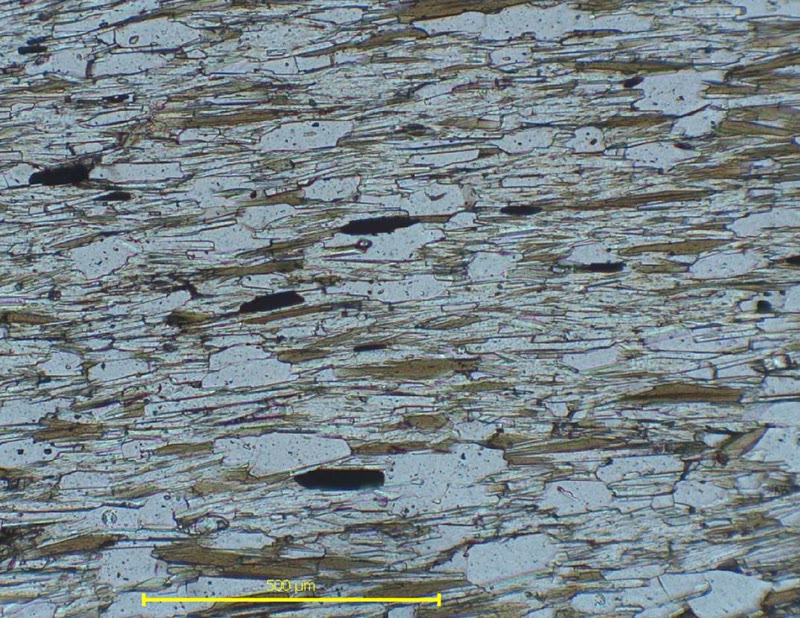
\includegraphics[height=4.3cm]{images/book2/g12-geoloshe-slaty-cleavage.jpg}\hspace{0.03\linewidth}%
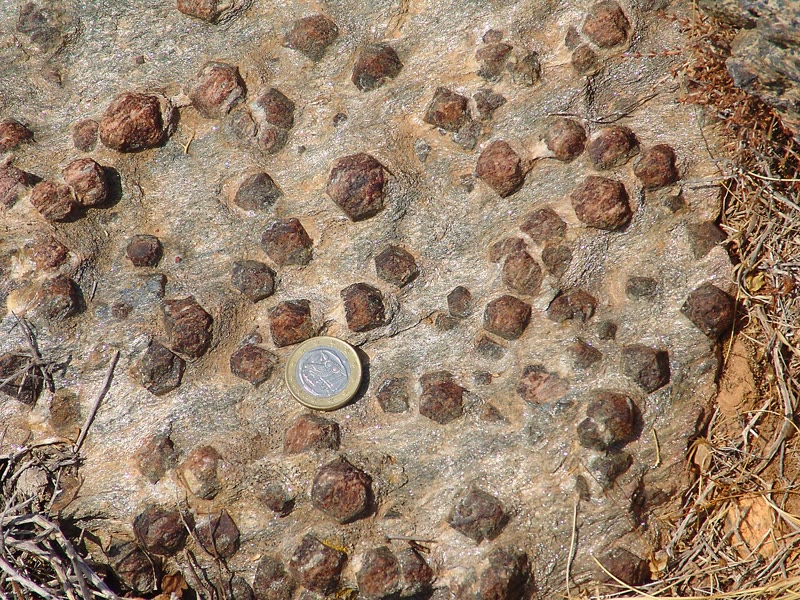
\includegraphics[height=4.3cm]{images/book2/g12-churchard-syros-garnet-schist.jpg}

\smallskip
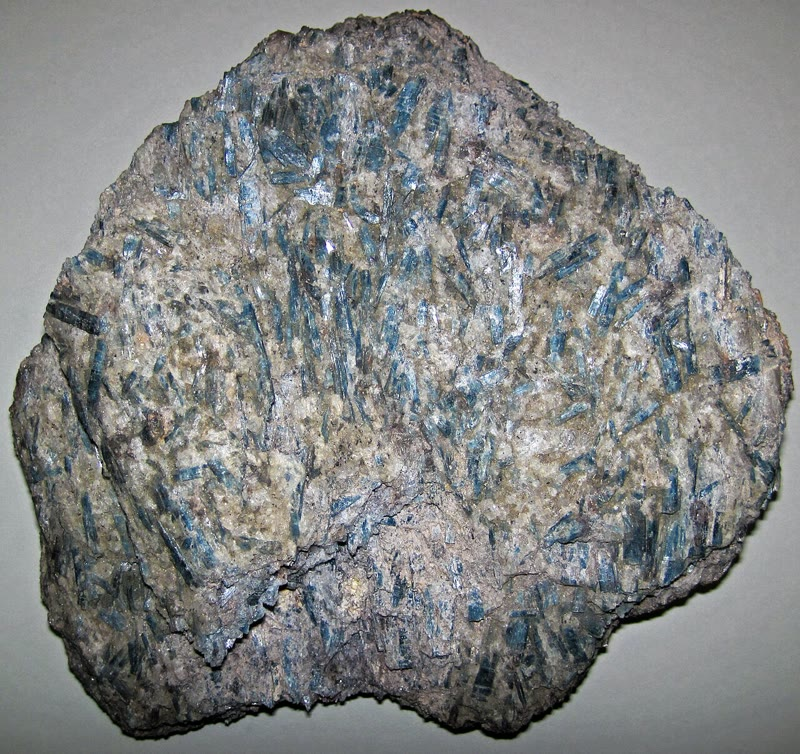
\includegraphics[height=4.3cm]{images/book2/g12-stjohn-kyanite-schist.jpg}\hspace{0.03\linewidth}%
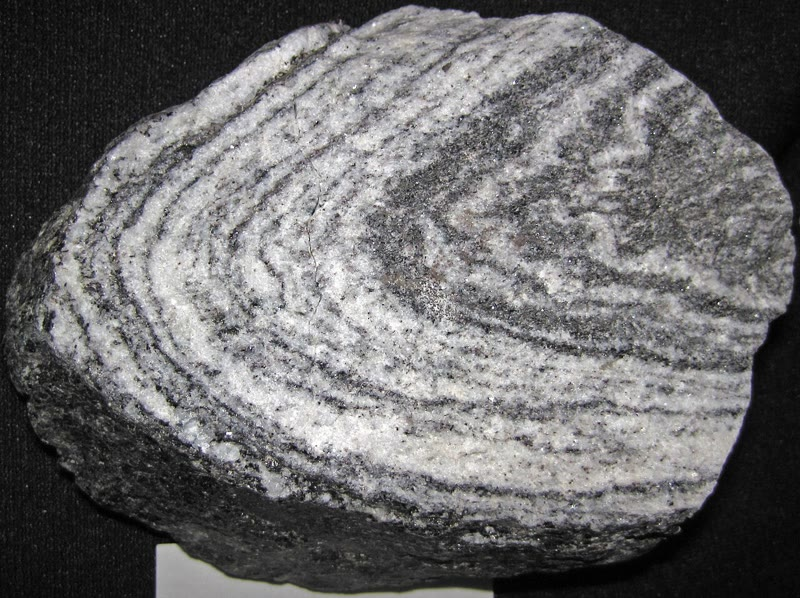
\includegraphics[height=4.3cm]{images/book2/g12-stjohn-gneiss.jpg}

{\small 左上：显微镜下的板岩（黄色标尺长
\qty{500}{\micro\metre}）：其云母\omterm{def:g11:minerals:thin-section}{薄片}方向一致。
右上：锡罗斯岛上的石榴石云母片岩，硬币直径
为\qty{23}{mm}。左下：一块带有蓝色刀片状蓝晶石的片岩。
右下：一块片麻岩，带有石英（浅色）与黑云母
（深色）条带。照片：Geoloshe（CC0）、Graeme Churchard（CC~BY~2.0）和 James
St.~John（CC~BY~2.0）。}
\end{omfigure}
% ledger: photo:g12-slaty-cleavage, photo:g12-syros-schist, photo:g12-kyanite-schist, photo:g12-gneiss

沿典型\omterm{def:g11:lithosphere-asthenosphere:geotherm}{地温线}，板岩形成于地下约 5 至 \qty{10}{km}
之间，千枚岩形成于 10 至 15，片岩形成于 15 至 20，
片麻岩形成于 20 至 \qty{25}{km} 之间；更深处，岩石局部开始熔化。
\omterm{def:g12:metamorphic-rocks:foliation}{面理}记录了挤压的方向：它垂直于造山缩短（
见\cref{ch:g12:mountain-building}）的方向形成，泥中原有的层理
仍可能以一定夹角与之相交。
% ledger: earle:settings, earle:foliation

不含扁平或细长矿物的岩石，即使受挤压也不显示\omterm{def:g12:metamorphic-rocks:foliation}{面理}。石灰岩
变为\textbf{大理岩}，由较大的方解石晶体组成，其中化石已被抹去；砂岩
变为\textbf{石英岩}，石英颗粒彼此长在一起；泥若只受加热而未受挤压，
则变为坚硬的细粒岩石，
无\omterm{def:g12:metamorphic-rocks:foliation}{面理}，
即\textbf{角岩}。
% ledger: earle:foliation, earle:contact

\section{接触变质作用与区域变质作用}

\begin{definition}[接触变质作用；区域变质作用；接触变质晕]\label{def:g12:metamorphic-rocks:contact-regional}
\emph{接触变质作用}\index{接触变质作用}是指被侵入的岩浆体加热的岩石
所发生的\omterm{def:g12:metamorphic-rocks:metamorphism}{变质作用}；它局限于\omterm{def:g11:igneous-rocks:intrusion}{侵入体}周围的一个带内，
即其\emph{接触变质晕}\index{接触变质晕}，其中\omterm{def:g12:metamorphic-rocks:index-mineral}{变质级}
向接触面升高。\emph{区域
变质作用}\index{区域变质作用}影响深埋于
大片区域的岩石，多见于板块汇聚处；岩石既受加热，也受挤压，
且几乎都具有\omterm{def:g12:metamorphic-rocks:foliation}{面理}。
\end{definition}
% ledger: earle:contact, earle:regional, tulane:metamorphism

\subsection{岩浆体周围}

温度约 \qty{1000}{\celsius} 的岩浆体上升进入冷的上地壳，加热周围的
岩石，其温度可达 300 至 \qty{800}{\celsius} 以上，
在浅部的低压条件下。\omterm{def:g12:metamorphic-rocks:contact-regional}{接触变质晕}很窄：围绕薄层岩浆体
仅数厘米宽，围绕大型岩体可达数十米。
这些岩石受热而未受挤压，因此不具\omterm{def:g12:metamorphic-rocks:foliation}{面理}：泥
变为角岩，石灰岩变为大理岩，砂岩变为石英岩。
侵位于本已炽热的深部岩石中的岩浆体，
几乎不形成\omterm{def:g12:metamorphic-rocks:contact-regional}{接触变质晕}。
% ledger: earle:contact, earle:settings (magma bodies around 1000 degC)

\begin{omfigure}
\begin{tikzpicture}[font=\scriptsize]
  \def\pluton{(3.0,0) .. controls (3.0,2.3) and (7.0,2.3) .. (7.0,0) -- cycle}
  \def\aureole{(2.45,0) .. controls (2.45,2.95) and (7.55,2.95) .. (7.55,0) -- cycle}
  \fill[lith sandstone] (0,0) rectangle (10,0.8);
  \fill[lith limestone] (0,0.8) rectangle (10,1.6);
  \fill[lith shale] (0,1.6) rectangle (10,3);
  \fill[omThm, opacity=0.30] \aureole;
  \draw[omThm, line width=0.6pt, dashed] (2.45,0) .. controls (2.45,2.95) and (7.55,2.95) .. (7.55,0);
  \fill[lith granite] \pluton;
  \draw[black!70, line width=0.6pt] (3.0,0) .. controls (3.0,2.3) and (7.0,2.3) .. (7.0,0);
  \draw[black!60] (0,0) rectangle (10,3);
  \node[fill=white, inner sep=1.5pt] at (5,0.45) {花岗岩（原为岩浆）};
  \draw[black!70] (6.0,1.95) -- (10.6,2.4) node[right] {角岩（由泥形成）};
  \draw[black!70] (7.0,1.2) -- (10.6,1.2) node[right] {大理岩（由石灰岩形成）};
  \draw[black!70] (7.25,0.4) -- (10.6,0.4) node[right] {石英岩（由砂岩形成）};
  \node[left] at (0,2.3) {页岩};
  \node[left] at (0,1.2) {石灰岩};
  \node[left] at (0,0.4) {砂岩};
  \draw[omThm] (4.2,2.05) -- (3.4,3.25) node[above, omThm] {接触变质晕};
\end{tikzpicture}

{\small \omterm{def:g12:metamorphic-rocks:contact-regional}{接触变质作用}剖面示意：岩浆体侵入层状沉积岩，
并加热其周围一条狭窄的\omterm{def:g12:metamorphic-rocks:contact-regional}{接触变质晕}（红色），该处岩石
在未受挤压的情况下发生重结晶。仅为示意：
实际\omterm{def:g12:metamorphic-rocks:contact-regional}{接触变质晕}宽数厘米至数十米。}
\end{omfigure}
% ledger: earle:contact

\subsection{造山带之下}

\omterm{def:g12:metamorphic-rocks:contact-regional}{区域变质作用}需要埋深达 10 至 \qty{20}{km}，因此
一次便影响数千平方千米的范围。最可能的场所是造山带的根部，
那里碰撞使地壳增厚，并将岩石向下推挤
（见\cref{ch:g12:mountain-building}）。在一条已测绘出各变质带的古老造山带中，
夕线石带的岩石被加热至 \qty{700}{\celsius} 以上，
并埋深达 20 至 \qty{25}{km}，而外侧绿泥石带的岩石
可能从未埋深超过约 \qty{5}{km}。其上的山脉随后在数千万年间遭受剥蚀，
载荷移除后，增厚的地壳重新抬升，
原先埋藏很深的各带如今出露于地表
（见\cref{ch:g12:destruction-of-mountains}）。
% ledger: earle:regional

\subsection{三条地温线}

\omterm{def:g12:metamorphic-rocks:polymorph}{同质多象变体}图一目了然地表明，相同深度处
并不一定对应同一种岩石，而取决于\omterm{def:g11:lithosphere-asthenosphere:geotherm}{地温线}。\omterm{def:g12:metamorphic-rocks:polymorph}{同质多象变体}图中
绘有三条\omterm{def:g11:lithosphere-asthenosphere:geotherm}{地温线}。
% ledger: earle:settings

\begin{itemize}
  \item 一条\textbf{典型}\omterm{def:g11:lithosphere-asthenosphere:geotherm}{地温线}，约为每千米 \qty{30}{\celsius}，
        在 \qty{10}{km} 深处温度约达 \qty{300}{\celsius}。
        该线经过三相点下方，因此蓝晶石直接转变为
        夕线石，转变条件约为 \qty{574}{\celsius} 和
        \qty{18.8}{km}。
  \item 一条\textbf{火山区}的\omterm{def:g11:lithosphere-asthenosphere:geotherm}{地温线}，约为每千米 40 至 \qty{50}{\celsius}，
        因上升岩浆的热量而变陡：岩石在较浅深度即
        可达到高温。当梯度为每千米 \qty{50}{\celsius} 时，
        红柱石约在 \qty{6.6}{km} 处出现，
        并在约 \qty{10.9}{km}、\qty{553}{\celsius} 处转变为夕线石。
  \item \textbf{\omterm{def:g11:subduction-zones:subduction}{俯冲带}}的\omterm{def:g11:lithosphere-asthenosphere:geotherm}{地温线}，低于每千米 \qty{10}{\celsius}：
        被\omterm{def:g11:subduction-zones:subduction}{俯冲}下去的\omterm{def:g11:ocean-ridges:oceanic-lithosphere}{洋壳}，比周围的地幔仍低数百度。在
        \qty{36}{km} 深处，温度仅约 \qty{370}{\celsius}，
        处于蓝晶石稳定区深部。这是一条低温高压路径，
        玄武岩沿此路径先变为\omterm{def:g11:subduction-zones:eclogite}{蓝片岩}，
        再于约 \qty{35}{km} 深处变为\omterm{def:g11:subduction-zones:eclogite}{榴辉岩}。
\end{itemize}
% values: cross_30_0 573.6 degC 18.79 km; cross_50_0 340.1 degC 6.60 km; cross_50_1 553.0 degC 10.86 km; sub10_T_at_1gpa 370.2 (al2sio5.py)
% ledger: earle:settings

因此，每种变质岩都记录着形成时的\omterm{def:g11:lithosphere-asthenosphere:geotherm}{地温线}及背后的板块构造背景：
红柱石和角岩指示岩浆体周围浅部的高温；
蓝晶石和夕线石片岩、片麻岩指示造山带的深部根部；
\omterm{def:g11:subduction-zones:eclogite}{蓝片岩}和\omterm{def:g11:subduction-zones:eclogite}{榴辉岩}则指示\omterm{def:g11:subduction-zones:subduction}{俯冲带}。
大多数此类岩石之所以能被观察到，
是因为它们回到地表时未再逆向变化。
岩石上升并冷却时，反应速率减慢，
而逆向反应所需的水已在下沉过程中逸出。
% ledger: earle:settings, earle:contact, tulane:metamorphism (retrograde metamorphism uncommon)

\section{练习}

\begin{exercise}[$\star$]\label{exo:g12:metamorphic-rocks:1}
写出下列各项对应的术语：（a）成分相同而晶体\omterm{def:g11:igneous-rocks:texture}{结构}不同的矿物；
（b）地图上\omterm{def:g12:metamorphic-rocks:index-mineral}{指示矿物}首次出现的界线；（c）岩浆体周围受热的岩石带；
（d）扁平矿物定向排列形成的平行面；
（e）由上覆岩石的
重量所产生的压力。
\end{exercise}

\begin{exercise}[$\star$]\label{exo:g12:metamorphic-rocks:2}
写出各\omterm{def:g10:soil-formation:weathering-profile}{母岩}变质后形成的变质岩名称：（1）石灰岩；
（2）砂岩；（3）泥，在低\omterm{def:g12:metamorphic-rocks:index-mineral}{变质级}且受挤压时；（4）泥，在高\omterm{def:g12:metamorphic-rocks:index-mineral}{变质级}时；
（5）泥，受岩浆体加热但未受挤压。
\end{exercise}

\begin{exercise}[$\star$]\label{exo:g12:metamorphic-rocks:3}
已知 $\rho = \qty{2830}{kg/m^3}$，$g = \qty{9.81}{m/s^2}$，计算
在 \qty{10}{km} 和 \qty{20}{km} 深度处的\omterm{def:g12:metamorphic-rocks:lithostatic}{静岩压力}，并以 \unit{GPa} 为单位。
\end{exercise}

\begin{exercise}[$\star$]\label{exo:g12:metamorphic-rocks:4}
根据 \ce{Al2SiO5} \omterm{def:g12:metamorphic-rocks:polymorph}{同质多象变体}的相图，哪种矿物在下列条件下稳定：
（1）在 \qty{400}{\celsius} 和 \qty{0.6}{GPa} 下；（2）在 \qty{500}{\celsius}
和 \qty{0.2}{GPa} 下；（3）在 \qty{750}{\celsius} 和 \qty{0.3}{GPa} 下？
\end{exercise}

\begin{exercise}[$\star$]\label{exo:g12:metamorphic-rocks:5}
（1）按\omterm{def:g12:metamorphic-rocks:index-mineral}{变质级}由低到高排列：片岩、板岩、片麻岩、千枚岩；（2）
其中哪些岩石的云母可用肉眼看到？
（3）哪一种岩石呈现明暗相间的条带？
\end{exercise}

\begin{exercise}[$\star\star$]\label{exo:g12:metamorphic-rocks:6}
（1）计算厚度为 \qty{35}{km} 的地壳底部的\omterm{def:g12:metamorphic-rocks:lithostatic}{静岩压力}
（$\rho = \qty{2830}{kg/m^3}$），并用大气压表示
（$\qty{1}{atm} = \qty{101325}{Pa}$）；（2）计算水深为 \qty{4}{km} 的
海底所受的压强，海水密度为
\qty{1025}{kg/m^3}；（3）前者是后者的多少倍？
\end{exercise}

\begin{exercise}[$\star\star$]\label{exo:g12:metamorphic-rocks:7}
\ce{Al2SiO5} 的三相点位于 \qty{504}{\celsius}、
\qty{0.375}{GPa} 处。（1）达到该压强的深度为多少（$\rho =
\qty{2830}{kg/m^3}$）？（2）从地表 \qty{10}{\celsius} 出发，
恰好经过该点的\omterm{def:g11:lithosphere-asthenosphere:geotherm}{地温梯度}为多少？（3）同时含三种\omterm{def:g12:metamorphic-rocks:polymorph}{同质多象变体}的岩石
是否常见？
\end{exercise}

\begin{exercise}[$\star\star$]\label{exo:g12:metamorphic-rocks:8}
在锡罗斯岛石榴子石片岩的照片中，最大的石榴子石直径约为
硬币直径的三分之一，而该硬币直径为 \qty{23}{mm}。（1）估算其直径；
（2）若石榴子石直径每一百万年约增长 \qty{1}{mm}，
则其生长用了多长时间？
（3）这对岩石在深处停留的时间说明了什么？
\end{exercise}

\begin{exercise}[$\star\star$]\label{exo:g12:metamorphic-rocks:9}
一位地质学家沿古老造山带向西步行 \qty{24}{km}，
记录下由泥形成的岩石。起始处的岩石只含绿泥石和黑云母，
行进 \qty{6}{km} 后首次出现石榴子石，行进 \qty{11}{km} 后首次出现十字石，
行进 \qty{15}{km} 后首次出现蓝晶石，行进
\qty{20}{km} 后首次出现夕线石。（1）穿过了几条\omterm{def:g12:metamorphic-rocks:index-mineral}{等变质线}？请按顺序写出其名称。
（2）\omterm{def:g12:metamorphic-rocks:index-mineral}{变质级}沿哪个方向升高？（3）岩石埋藏最深处在哪里？
那里的温度大致达到多少？
\end{exercise}

\begin{exercise}[$\star\star$]\label{exo:g12:metamorphic-rocks:10}
一团岩浆在地表附近侵入泥、石灰岩和砂岩
的岩层中。（1）写出各岩层紧邻岩浆处所变成的岩石名称。（2）这些
岩石为何不具\omterm{def:g12:metamorphic-rocks:foliation}{面理}？（3）第二团岩浆侵位于地下 \qty{20}{km} 深处，
围岩温度已接近 \qty{500}{\celsius}，为何几乎不形成\omterm{def:g12:metamorphic-rocks:contact-regional}{接触变质晕}？
\end{exercise}

\begin{exercise}[$\star\star$]\label{exo:g12:metamorphic-rocks:11}
碰撞期间，一层泥受到来自东西两侧的挤压，
受热时生长出云母。（1）云母如何排列：其片状面
朝向东–西方向还是南–北方向？（2）形成的\omterm{def:g12:metamorphic-rocks:foliation}{面理}
是水平的还是竖直的？（3）以相同方式挤压的大理岩和石英岩
均不显示\omterm{def:g12:metamorphic-rocks:foliation}{面理}，为什么？
\end{exercise}

\begin{exercise}[$\star\star\star$]\label{exo:g12:metamorphic-rocks:12}
在 500 至 \qty{700}{\celsius} 之间，蓝晶石–夕线石边界
近似为直线 $P = 0.577 + 0.00209\,(T - 600)$，其中 $P$ 以
\unit{GPa}、$T$ 以 \unit{\celsius} 为单位。典型\omterm{def:g11:lithosphere-asthenosphere:geotherm}{地温线}为 $T = 10 + 30z$
（$z$ 以 \unit{km} 为单位），且 $P = 0.0278\,z$。（1）将\omterm{def:g11:lithosphere-asthenosphere:geotherm}{地温线}写成 $P$ 关于
$T$ 的函数。（2）求\omterm{def:g11:lithosphere-asthenosphere:geotherm}{地温线}与边界线的交点：温度、压强、
深度。（3）沿此\omterm{def:g11:lithosphere-asthenosphere:geotherm}{地温线}，在该深度以浅处稳定的是哪种\omterm{def:g12:metamorphic-rocks:polymorph}{同质多象变体}，
在其以深处又是哪种？
\end{exercise}

\begin{exercise}[$\star\star\star$]\label{exo:g12:metamorphic-rocks:13}
（1）沿每千米升温 \qty{10}{\celsius} 的\omterm{def:g11:subduction-zones:subduction}{俯冲}\omterm{def:g11:lithosphere-asthenosphere:geotherm}{地温线}，从 \qty{10}{\celsius} 出发，
求 \qty{35}{km} 深处（\omterm{def:g11:subduction-zones:eclogite}{榴辉岩}形成处）的温度。（2）沿典型\omterm{def:g11:lithosphere-asthenosphere:geotherm}{地温线}
（每千米升温 \qty{30}{\celsius}），该处温度为多少？（3）将两点
标注在\omterm{def:g12:metamorphic-rocks:polymorph}{同质多象变体}图上，第一点处稳定的是哪种\omterm{def:g12:metamorphic-rocks:polymorph}{同质多象变体}？（4）为何
\omterm{def:g11:subduction-zones:eclogite}{蓝片岩}和\omterm{def:g11:subduction-zones:eclogite}{榴辉岩}几乎只在\omterm{def:g11:subduction-zones:subduction}{俯冲带}中形成，
而很少在其他地方形成？
\end{exercise}

\begin{exercise}[$\star\star\star$]\label{exo:g12:metamorphic-rocks:14}
蓝晶石、夕线石和红柱石的密度分别为 \num{3.61}、
\num{3.24} 和 \qty{3.15}{g/cm^3}。（1）计算 \qty{1}{kg} 各矿物的体积，
单位为 \unit{cm^3}。（2）质量相同时，蓝晶石的体积比红柱石小百分之几？
（3）利用“高压有利于占据空间最小的排列”这一观点，
解释为何蓝晶石占据图中的
高压区域。
\end{exercise}

\begin{exercise}[$\star\star\star$]\label{exo:g12:metamorphic-rocks:15}
在一条古老的造山带中，夕线石带的岩石被加热至超过
\qty{700}{\celsius}，并埋藏于 20 至 \qty{25}{km} 深处。（1）计算
深度为 20 和 \qty{25}{km} 处的压强。（2）利用
习题 12 中的直线，求夕线石在这两个压强下稳定的最低温度。
\qty{700}{\celsius} 是否与夕线石相容？（3）从地表 \qty{10}{\celsius} 出发，
要使 \qty{700}{\celsius} 分别出现在 20 和 \qty{25}{km} 深处，需要怎样的\omterm{def:g11:lithosphere-asthenosphere:geotherm}{地温梯度}？
（4）这些岩石约在
4000 万年后出露于地表。其上覆岩石被剥蚀的平均速率是多少，
单位以 \unit{mm} 每年计？
\end{exercise}

\begin{problem}[{周末问题——一块蓝晶石片岩的历史}]
\label{pb:g12:metamorphic-rocks:1}
% ledger: hm93:table11, cm95:crust, earle:controls, earle:settings, earle:regional, tulane:roots, tulane:metamorphism, iugs:barrow; Book 3: webmineral:polymorphs; Book 1: ussa76:sea-level
% values: pb_z_km 25.214, pb_grad 23.4, pb_kysil_P_at_600_gpa 0.577 (al2sio5.py); t_on_kysil(7.0) = 658.9
在一条古老造山带的核部采集到一块片岩，其中含白云母、
黑云母、石英、直径可达 \qty{8}{mm} 的石榴子石，以及蓝色刀片状的
蓝晶石；其中既不含夕线石，也不含红柱石。对其石榴子石和黑云母的实验室分析表明，
它的结晶条件约为
\qty{600}{\celsius} 和 \qty{0.70}{GPa}。取 $\rho =
\qty{2830}{kg/m^3}$，$g = \qty{9.81}{m/s^2}$，地表温度为 \qty{10}{\celsius}，
并取习题 12 中的蓝晶石–夕线石直线 $P = 0.577 +
0.00209\,(T - 600)$.

\medskip
\noindent\textbf{第一部分——矿物。}
\begin{enumerate}
  \item 该岩石为何被称为片岩？其中哪些矿物形成了
        \omterm{def:g12:metamorphic-rocks:foliation}{片理}？
  \item 蓝晶石、红柱石和夕线石具有相同的化学式。写出该化学式，并
        说出这类矿物的名称。
  \item 蓝晶石和红柱石的密度分别为 \num{3.61} 和
        \qty{3.15}{g/cm^3}。一千克蓝晶石的体积
        小百分之几？压强有利于哪一种矿物？
  \item 在由泥形成的岩石的\omterm{def:g12:metamorphic-rocks:index-mineral}{指示矿物}序列中，该岩石
        属于哪一变质带？它在埋藏过程中穿过了哪些\omterm{def:g12:metamorphic-rocks:index-mineral}{等变质线}？
  \item 若石榴子石的直径在一百万年内约增长 \qty{1}{mm}，
        则最大的石榴子石需要多长时间才能长成？
\end{enumerate}

\medskip
\noindent\textbf{第二部分——压强与温度。}
\begin{enumerate}[resume]
  \item 在 \qty{600}{\celsius} 时，压强超过多少时蓝晶石
        而非夕线石稳定？
  \item 检验点 (\qty{600}{\celsius}, \qty{0.70}{GPa}) 是否位于
        蓝晶石稳定区内。
  \item 夕线石的缺失给出了在
        \qty{600}{\celsius} 时的一个最低压强。该压强为多少？
  \item 若岩石在 \qty{0.70}{GPa} 下继续加热，
        温度达到多少时其中的蓝晶石会转变为夕线石？
  \item 将 \qty{0.70}{GPa} 分别用千巴（$\qty{1}{kbar} =
        \qty{e8}{Pa}$）和标准大气压（$\qty{1}{atm} = \qty{101325}{Pa}$）表示。
\end{enumerate}

\medskip
\noindent\textbf{第三部分——埋藏深度。}
\begin{enumerate}[resume]
  \item \omterm{def:g12:metamorphic-rocks:lithostatic}{静岩压力}每
        千米升高多少兆帕？
  \item 该片岩结晶时位于多深处？
  \item 夕线石缺失所允许的最小深度是多少
        （第 8 题）？
  \item 取上覆岩石的密度为 \qty{2700}{kg/m^3}，重做第 12 题，
        深度变化了百分之几？
  \item \omterm{def:g12:continental-crust:continental-crust}{大陆地壳}通常厚 35 至 \qty{40}{km}，造山带之下厚 50 至
        \qty{70}{km}。该片岩是在地壳中还是
        地幔中结晶的？
\end{enumerate}

\medskip
\noindent\textbf{第四部分——\omterm{def:g11:lithosphere-asthenosphere:geotherm}{地温线}与折返。}
\begin{enumerate}[resume]
  \item 在该深度达到 \qty{600}{\celsius} 意味着
        怎样的平均\omterm{def:g11:lithosphere-asthenosphere:geotherm}{地温梯度}？
  \item 将其与\omterm{def:g11:subduction-zones:subduction}{俯冲带}、典型地壳和火山区的\omterm{def:g11:lithosphere-asthenosphere:geotherm}{地温梯度}进行比较，
        该岩石是哪一类\omterm{def:g12:metamorphic-rocks:metamorphism}{变质作用}形成的？
  \item 沿每千米升温 \qty{30}{\celsius} 的典型\omterm{def:g11:lithosphere-asthenosphere:geotherm}{地温线}，
        第 12 题所指深度处的温度将是多少？
        此时在 \qty{0.70}{GPa} 下稳定的是哪种\omterm{def:g12:metamorphic-rocks:polymorph}{同质多象变体}？
  \item 要使该片岩出露于地表，其上覆的全部岩石
        都须被剥蚀。若平均速率为 \qty{0.5}{mm} 每年，
        这一过程需要多长时间？
  \item 蓝晶石在折返过程中为何没有转变回红柱石？
  \item 总结：这块蓝晶石片岩是在多深处结晶的？
\end{enumerate}
\end{problem}
